%%%%%%%%%%%%%%%%%%%%%%%%%%%%%%%%%%%%%%%%%%%%%%%%%%%%%%%%%%%%%%%%%%%%%%
%     File: ExtendedAbstract_imple.tex                               %
%     Tex Master: ExtendedAbstract.tex                               %
%%%%%%%%%%%%%%%%%%%%%%%%%%%%%%%%%%%%%%%%%%%%%%%%%%%%%%%%%%%%%%%%%%%%%%

\section{Aerial-D Dataset Construction}
\label{sec:approach}

\subsection{Rule-Based Expression Generation}

\begin{figure*}[t]
\centering
\begin{minipage}{0.5\textwidth}
\centering
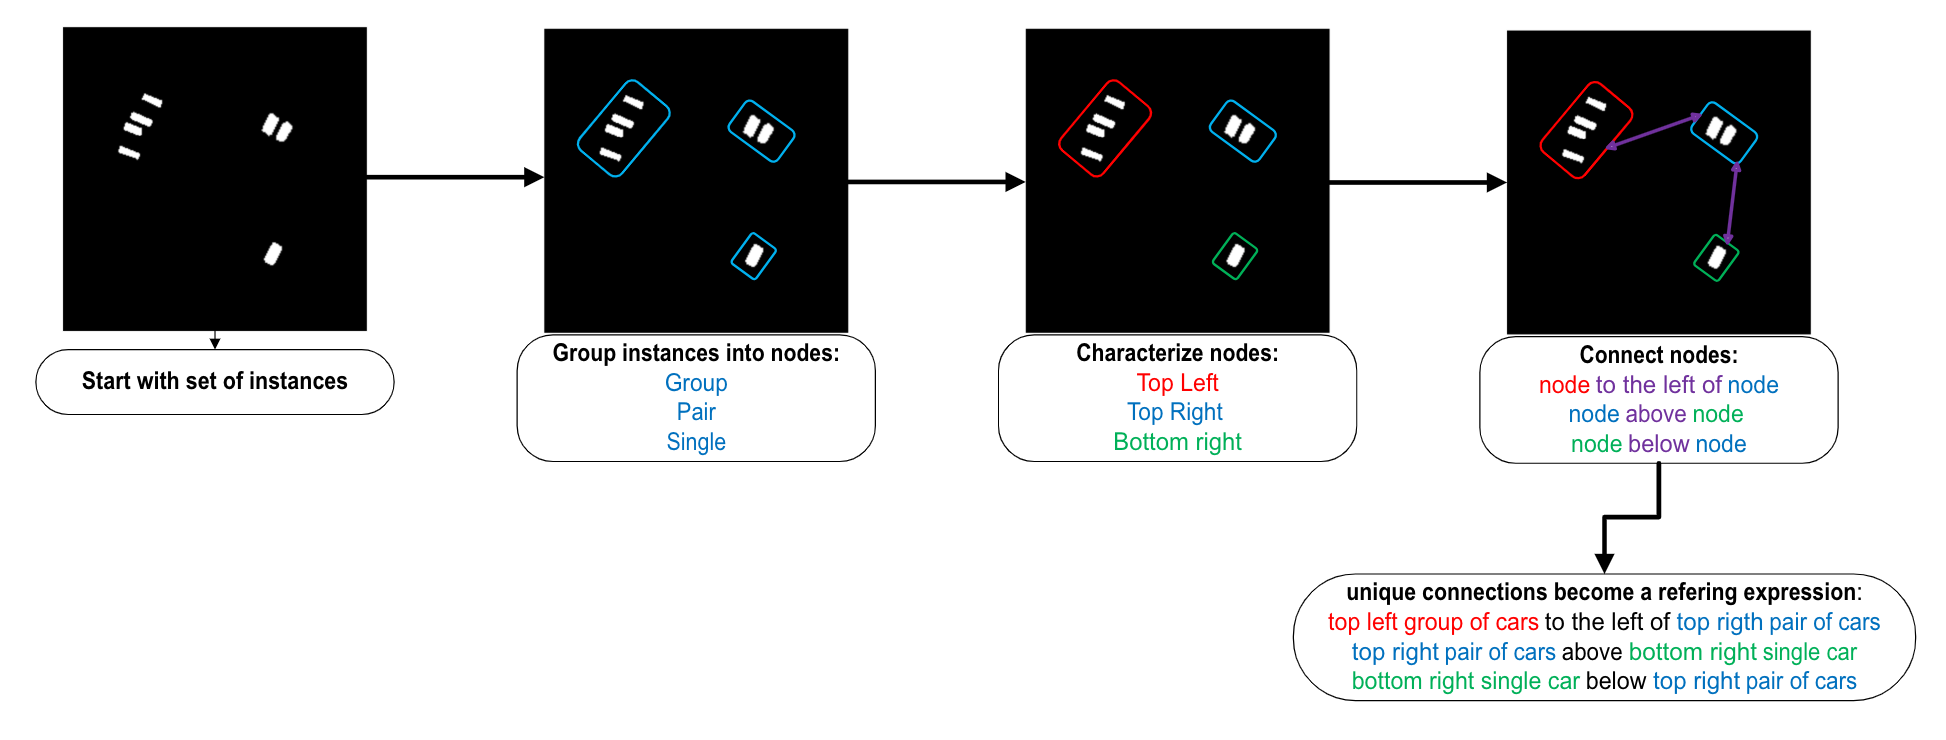
\includegraphics[width=0.7\textwidth]{./images/rule_based_generation.png}
\end{minipage}%
\begin{minipage}{0.5\textwidth}
\centering
\hspace{-1cm}
\raisebox{-0.3\height}{%
\resizebox{\textwidth}{!}{%
\footnotesize
\begin{tabular}{@{}ll@{}}
\toprule
\textbf{Rule Type} & \textbf{Example Instance} \\
\midrule
Category & "plane" \\
Grid Position & "in the top right" \\
Extreme Position & None \\
Color Classification & "light" \\
Directional Relations & "to the bottom right of a plane" \\
& "to the top right of a plane" \\
\midrule
\multicolumn{2}{l}{\textbf{Final Expressions}} \\
\multicolumn{2}{l}{"the plane in the top right"} \\
\multicolumn{2}{l}{"the light plane in the top right"} \\
\multicolumn{2}{l}{"the plane in the top right to the bottom right of a plane"} \\
\multicolumn{2}{l}{"the light plane in the top right to the bottom right of a plane"} \\
\multicolumn{2}{l}{"the plane in the top right to the top right of a plane"} \\
\multicolumn{2}{l}{"the light plane in the top right to the top right of a plane"} \\
\bottomrule
\end{tabular}%
}%
}
\end{minipage}
\caption{Example of rule generation for a single instance. The highlighted plane in the top right section demonstrates how the system assigns spatial, visual, and relational rules that will later be combined into referring expressions.}
\label{fig:rule_example}
\end{figure*}


\subsection{LLM Expression Generation}

\begin{figure*}[t]
\centering
\begin{minipage}{0.5\textwidth}
\centering
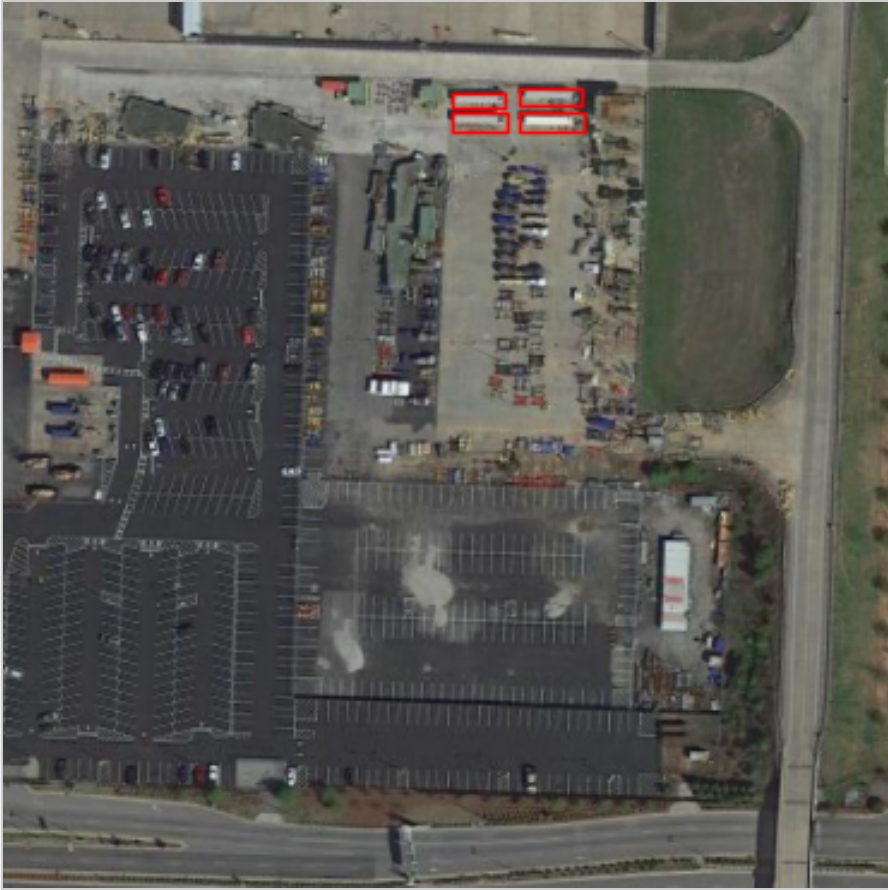
\includegraphics[width=0.7\textwidth]{./images/example_group.png}
\end{minipage}%
\begin{minipage}{0.5\textwidth}
\centering
\hspace{-1cm}
\raisebox{-0.3\height}{%
\footnotesize
\begin{tabular}{@{}p{2cm}p{5cm}@{}}
\toprule
\textbf{Expression Type} & \textbf{Example} \\
\midrule
Original & the group of 4 large vehicles in the top center \\
\midrule
Enhanced & the cluster of four big vehicles near the upper middle \\
\midrule
Unique & the four large vehicles lined up side by side just below the pale paved strip at the very top middle \\
\midrule
Unique & the set of four big vehicles parked in a single row in the upper center beside the grassy area to the right \\
\bottomrule
\end{tabular}%
}
\end{minipage}
\caption{Example of LLM enhancement process showing original aerial image with group of four large vehicles (left) and corresponding expression enhancements (right).}
\label{fig:llm_enhancement_example}
\end{figure*}


\begin{figure}[H]
\centering
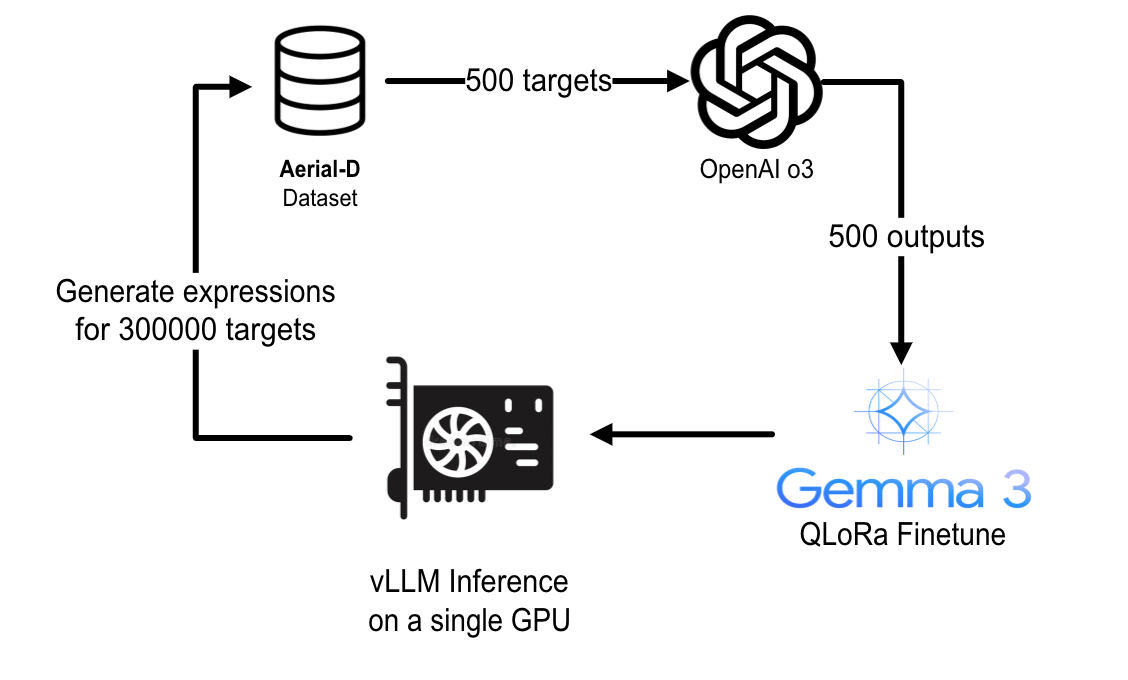
\includegraphics[width=0.8\columnwidth]{./images/distillation.png}
\caption{Knowledge distillation pipeline for scalable LLM enhancement. A small sample of 500 expressions is processed through OpenAI's O3 model to generate high-quality training targets, which are then used to fine-tune Gemma3 12B via QLora. The fine-tuned model enables cost-effective local inference to enhance the full dataset of 300,000 expressions using vLLM on a single GPU.}
\label{fig:llm_distillation}
\end{figure}
